\begin{figure}[htbp]
\centering
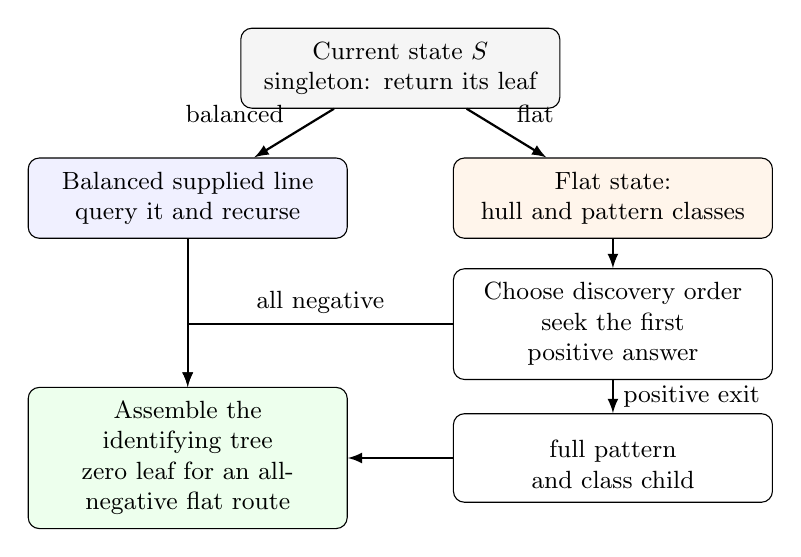
\begin{tikzpicture}[every node/.style={font=\small},
  box/.style={draw,rounded corners,align=center,inner sep=5pt,text width=3.7cm},
  arr/.style={-latex,thick}]
  \node[box,fill=gray!8] (state) at (0,0) {Current state $S$\\singleton: return its leaf};
  \node[box,fill=blue!6] (balanced) at (-2.7,-1.65)
    {Balanced supplied line\\query it and recurse};
  \node[box,fill=orange!8] (flat) at (2.7,-1.65)
    {Flat state: \HullData\\hull and pattern classes};
  \node[box] (discover) at (2.7,-3.25)
    {Choose discovery order\\seek the first positive answer};
  \node[box] (decode) at (2.7,-4.95)
    {\EndpointCode\\full pattern and class child};
  \node[box,fill=green!7] (output) at (-2.7,-4.95)
    {Assemble the identifying tree\\zero leaf for an all-negative flat route};
  \draw[arr] (state) -- node[above left]{balanced} (balanced);
  \draw[arr] (state) -- node[above right]{flat} (flat);
  \draw[arr] (flat) -- (discover);
  \draw[arr] (discover) -- node[right]{positive exit} (decode);
  \draw[arr] (discover.west) -- node[above]{all negative} (-2.7,-3.25)
    -- (output.north);
  \draw[arr] (decode) -- (output);
  \draw[arr] (balanced) -- (output);
\end{tikzpicture}
\caption{The common recursive structure. Arrows show how one stage
feeds the next. For maximum depth, the algorithm constructs class
children first and uses their heights as schedule deadlines. For
expected depth, original prior masses determine the schedule scores.
The flat stage has an all-negative leaf when the zero pattern is
present, and both scheduling and decoding use supplied hull lines.}
\label{fig:recursive-procedure-flow}
\end{figure}

